

\subsection{Base Stock Model}


\subsubsection{Common notation}
\label{sec:common-notation}

Let $I_t$ denote the on-hand inventory at time $t$, $B_t$ the number
of backorders, $R_t$ the number of out-standing replenishments, and
$X_t := X(t-L,t]$ the demand that occurred during the time interval
$(t-L, t]$. Note that here we write $X_t$ to represent the
random variable $X$ of Factory Physics.
We also write
\begin{equation}
  \label{eq:16}
   G(r) = \P{X_t\leq r},
\end{equation}
and for the average demand during a lead time 
\begin{equation*}
\theta = \E{X_t}.
\end{equation*}

Under the basestock policy the above random variables $I_t, B_t, R_t$
and $X_t$ satisfy a number of important relations.  Recally that
according to the basestock policy we issue a replenishment order as
soon as the re-order level $r$ is hit. First, as for each demand a
replenishment order is sent, it must be that
\begin{equation}
  \label{eq:8}
   R_t = X(t-L, t] = X_t,
\end{equation}
that is, the number of outstanding replenishments at time $t$ equals
all demand $X_t$ that occurred during the previous leadtime.  
Second, as each demand spawns a replenishment, it must be for all time
$t$ that the on-hand inventory $I_t$ plus the number of
replenishments $R_t$ minus all backorders $B_t$ remains
constant. That is, 
\begin{equation*}
I_t + R_t - B_t = \text{ constant}.
\end{equation*}
Third, we do not backorder demand when there is on-hand stock and we
also match backorders (if any) with replenishments as they arrive, it
must hold that
\begin{equation}
  \label{eq:9}
   I_t B_t =0, \text{ for all }  t\geq 0.
\end{equation}
In other words, at any moment in time the on-hand inventory $I_t = 0$ or the
number of backorders $B_t=0$.

Assuming that at time $t=0$,
there are no outstanding replenishments and no backorders, we can
safely assume that $I_0 = r+1$. The above then implies that
\begin{equation}
  \label{eq:7}
   I_t + R_t - B_t = r+1, \text{ for all }  t\geq 0.
\end{equation}


When dealing with positive leadtimes two concepts are very useful. The \emph{inventory level} $\IL_t$ at time $t$ is the basestock level minus the demand: 
\begin{equation}\label{eq:23}
  \IL_t = r+1 - X_t
\end{equation}
Note that from~\eqref{eq:8} and~\eqref{eq:7} it follows that
\begin{equation*}
  \begin{split}
  \IL_t 
&=r - X_t \\
&= (I_t + R_t - B_t) - X_t \\
&= I_t - B_t.
  \end{split}
\end{equation*}


The \emph{inventory position} $\IP_t$ is the inventory level plus all outstanding replenishments:
\begin{equation*}
  \IP_t = \IL_t + R_t.
\end{equation*}
From \eqref{eq:7} we conclude that 
\begin{equation}\label{eq:20}
\IP_t =\IL_t + R_t = I_t - B_t +R_t = r+1.
\end{equation}
Thus, for the basestock mode in continuous time, the inventory position is constant. 

\begin{remark}
Below we develop a set of expressions for the most relevant KPIs such
as the service level. In Section~\ref{sec:qr_example-code} we provide some computer code on how to compute these KPIs. This code is not obligatory for the course. 
\end{remark}


\begin{question}
  What is the reorder level $r$ for a make-to-order inventory system?
\end{question}
\begin{solution}
  In a make-to-order setting, there is no on-hand
  inventory. Production starts when a job comes in. Thus, if we take
  $r=-1$, then when the inventory position hits $-1$, we issue a
  production order. Clearly, $I_t=0$ always, and $B_t$ is the number
  of jobs waiting to get served by production.
\end{solution}


\begin{question}\label{q:basestock}
  Suppose the demand during the leadtime is like this:
  \begin{align*}
    \P{X = 0} &= 1/6, & \P{X \leq 0} &= 1/6,  \\
    \P{X = 1} &= 1/5, & \P{X \leq 1} &= 11/30,  \\
    \P{X = 2} &= 1/4, & \P{X \leq 2} &= 37/60, \\
    \P{X = 3} &= 1/8, & \P{X \leq 3} &= 89/120, \\
    \P{X = 4} &= 11/120, & \P{X \leq 4} &= 5/6, \\
    \P{X = 5} &= 1/6, & \P{X \leq 5} &= 1.
  \end{align*}
What is $\theta$?
\end{question}
\begin{solution}
  \begin{equation*}
    \theta = \E{X} =
1\cdot 1/5 + \cdots + 5 \cdot 1/6 = 91/40.
  \end{equation*}
\end{solution}

\subsubsection{Computing the Service level}

The service level $S(r)$ is defined as the fraction of demand that
perceives, on arrival, a positive stock level. As we assume that demand
occurs in single units, this fraction is therefore equal to the fraction
of demand served from on-hand stock. We also assume that the arrival
process is given by a Poisson process. Therefore, by the PASTA property,
the fraction of demand served from stock is equal to the (long-run)
fraction of time that the inventory level is positive. Hence,
\begin{equation*}
   S(r) = \P{I_t >0}.
\end{equation*}

Using that $I_t>0$ at time $t$ implies that $B_t = 0$,
it follows from Eq.~\eqref{eq:7} that:
\begin{equation}\label{eq:10}
  \begin{split}
   S(r) &= \P{I_t >0} \\
   &= \P{r+1 + B_t - R_t >0}, \text{  from  \eqref{eq:7}}  \\
   &= \P{r+1 - R_t >0}, \text{ as } B_t = 0, \\
   &= \P{R_t < r+1} \\
   &= \P{R_t \leq r} \\
   & = \P{X_t \leq  r}, \text{from  \eqref{eq:8}}, \\
   &= G(r),  \text{ from \eqref{eq:16}} \\
   &=  \sum_{i=0}^{r} g_i.
  \end{split}
\end{equation}
Thus,
\begin{equation}
  \label{eq:13}
   S(r) = G(r) = \sum_{i=0}^r \P{X_t = i},
\end{equation}
and \emph{not} $G(r+1)$ as in the third edition of Factory Physics.


\begin{question}\label{q:basestock}
  Suppose the demand is a given by  Exercise~\ref{q:basestock}.
What is $S(r)$ for $r=0, \ldots, 5$?
\end{question}
\begin{solution}
  \begin{equation*}
    S(r) = G(r) = \sum_{i=0}^r \P{X = i}.
  \end{equation*}
Hence,
\begin{align*}
  r &= 0 \implies S(0) = \P{X \leq 0} = \P{X=0}1/6, \\
  r &= 1 \implies S(1) = \P{X \leq 1} = 1/6 + 1/5 = 11/33, \\
  r &= 2 \implies S(2) = \P{X \leq 2} = 37/60,\\
  r &= 3 \implies S(3) = 89/120, \\
  r &= 4 \implies S(4) = 100/120 = 5/6, \\
  r &= 5 \implies S(5) = 1.
\end{align*}
\end{solution}

\subsubsection{Computing the average backorder level}


When does a backorder occur? This happens whenever
\begin{equation}
  \label{eq:11}
  \begin{split}
   \{B_t > 0\} 
&= \{R_t - r-1>0\}, \quad \text{ as } R_t - B_t = r+1\text{ when } B_t >0, \\
&= \{X_t - r-1>0\},\quad \text{ since  } R_t  = X_t.
  \end{split}
\end{equation}
Hence,
\begin{equation*}
   \begin{split}
     B(r) 
   &= \E{B_t} \\
   &= \E{\max\{B_t, 0\}} \\
   &= \E{\max\{R_t - r - 1, 0\}} \\
   &= \E{\max\{X_t - r - 1, 0\}} \\
   &= \sum_{i=r+1}^\infty (i- r -1)\P{X_t = i}\\
   &= \sum_{i=r+1}^\infty (i- r -1)g_i \\
   &= \sum_{i=r+2}^\infty (i- r -1)g_i,
     \end{split}
\end{equation*}
where the last equation follows from the fact that when $i=r+1$,
$i-r-1 =0$. I find the following easier to memorize, hence I use this
in the sequel:
\begin{equation}
  \label{eq:12}
   B(r)  = \sum_{i=r+1}^\infty (i- r -1)g_i.
\end{equation}

Note that in the above formula for $B(r)$ the summation runs to $\infty$, which is a bit problematic for numerical purposes. In the proof below we show that this expression can be rewritten to 
\begin{equation}
  \label{eq:17}
   B(r) 
%= \sum_{i=r+1}^{\infty} \bar G(i)
   = \theta - \sum_{j=0}^{r} \bar G(j)
\end{equation}
where
\begin{equation}
  \label{eq:18}
   \bar G(i) = \P{X>i} = 1 - \P{X\leq i} = 1 - G(i),
\end{equation}
and $\theta = \E{X_t}$. You can skip the proof. 
\begin{proof}
Define first the function
\begin{equation*}
   \1{i< j} =
     \begin{cases}
       1, &\text{  if } i < j, \\
   0, &\text{ else},
     \end{cases}
\end{equation*}
so that we can write
\begin{equation*}
  \sum_{j=0}^\infty \1{j< i-r - 1} = i-r -1.
\end{equation*}
Now, using \eqref{eq:12},
\begin{equation}
  \label{eq:19}
  \begin{split}
       B(r) &= 
   \sum_{i=r+1}^\infty (i-r-1) g(i)   \\
   &= \sum_{i=r+1}^\infty\sum_{j=0}^\infty \1{j < i-r-1}\, g(i)   = 
    \sum_{j=0}^\infty \sum_{i=r+1}^\infty \1{i > j +r + 1}\, g(i)\\
   &= \sum_{j=0}^\infty \sum_{i=j + r+2}^\infty  g(i) = 
   \sum_{j=0}^\infty \P{X_t \geq j + r+2}  \\
   &=\sum_{j=0}^\infty \P{X_t > j + r+1} \\
   &= \sum_{j=0}^\infty \bar G(j+r+1) =\sum_{j=r+1}^\infty  \bar G(j).
  \end{split}
\end{equation}
Finally, this can be simplied a bit by using that
$\sum_{i=0}^\infty \bar G(i) = \theta$:
\begin{equation}
  \label{eq:119}
  \begin{split}
   B(r) 
   &= \sum_{j=r+1}^\infty  \bar G(j) \\
   &= \sum_{j=0}^\infty  \bar G(j) - \sum_{j=0}^{r} \bar G(j)\\
   &= \theta - \sum_{j=0}^{r} \bar G(j)
  \end{split}
\end{equation}
  
\end{proof}
	   

\begin{question}\label{q:basestock_B}
  Suppose the demand is a given by  Exercise~\ref{q:basestock}. What is $B(r)$ for $r=0,\ldots, 5$.?
\end{question}
\begin{solution}
  Use that $B(r) = \sum_{i=r+1}^\infty (i-r-1)g(i)$, and that $g(i) = \P{X = i}$, and that $g(i)=0$ for $i\geq 6$.
  \begin{align*}
    r&=0 \implies B(0) = \sum_{i=1}^\infty (i-1)g(i) =  0\cdot 1/5 + \cdots + 4 \cdot 1/6 = 173/120, \\
    r&=1 \implies B(1) = \sum_{i=2}^6 (i-2)g(i) =  1\cdot 1/8 + 2\cdot 11/120 + 3 \cdot 1/6 = 97/120, \\
    r&=2 \implies B(2) = 1\cdot 11/120 + 2 \cdot 1/6 = 17/40, \\
    r&=3 \implies B(3) = 1 \cdot 1/6 = 1/6, \\
  \end{align*}
\end{solution}


\subsubsection{Computing the expected on-hand inventory}

Taking expectations at the left and right hand side of \eqref{eq:7} we get
\begin{equation*}
  \E{I_t + R_t - B_t} = r+1,
\end{equation*}
from which we find for the on-hand inventory $I_t$: 
\begin{equation}
  \label{eq:6}
  \begin{split}
  \E{I_t}
  &= r+1 - \E{R_t} + \E{B_t}  \\
  & = r + 1 - \E{X_t} + B(r) \\
  & = r + 1 - \theta + B(r) \\
  \end{split}
\end{equation}

Formulas to skip (in edition 3): 2.24, 2.25. 

\begin{question}
Suppose the demand is a given by Exercise~\ref{q:basestock}. What is $I(r)$ for $r=0,\ldots, 5$.?
\end{question}
\begin{solution}
  Use that $I(r) = \E{I_t} = r+1-\theta + B(r)$.  The result follows straightaway from Exercise~\ref{q:basestock_B}. As an example
  \begin{equation*}
    I(3) = 3+1 - \theta + B(3) = 4 - 91/40 + 1/6 = 227/120.
  \end{equation*}
\end{solution}

\begin{question}
Suppose the demand is a given by the previous exercise and that the holding cost $h=1$ and the backlog cost per item is $b=5$.  What is $r$ that minimizes $hI(r)+bB(r)$?
\end{question}


\subsubsection{Simulation of the basestock inventory model}
\label{sec:simul-basest-invent}

Consider a periodic-time model so that $\IP_t$ is the inventory position at the end of period $t$. Write $D_t = X(t-1, t]$ for the demand that occured in period $t$. (Recall that $X_t = X(t-L, t]$ is the demand during the leadtime $L$, which is not the same as the demand during one period.)
 Then the sequence $\{\IP_i\}$ must satisfy the recursion:
\begin{equation}
  \label{eq:15}
  \IP_t = r+1 = r+1 - D_t + D_t \1{D_t>0} = r+1.
\end{equation}
To see this, observe that under the basestock policy the inventory
position is always kept at level $r+1$, c.f., \eqref{eq:20}. Thus, if
the inventory position $\IP_t$ at the end of period $t$ minus the demand
$D_t$ during period $t$ is less than $r+1$, we need to reorder to fill up the
shortage. Since the shortage is precisely the demand during period
$t$, i.e., $D_t$, we order $D_t$. 
% Finally, recall that the indicator function $\1{D_t>0} = 1$ if
% $D_i>0$ and is $0$ otherwise, so that this indicator is only positive when $D_t>0$, precisely as we want.  


When the leadtime $L$ is one period or more, the replenishments do not arrive right away but~$L$ periods later. The consequences for the inventory level are that
\begin{equation}
  \label{eq:21}
  \IL_t = \IL_{t-1} - D_t + D_{t-L}\1{D_{t-L}>0} = \IL_{t-1} - D_t + D_{t-L}.
\end{equation}
Thus, what we ordered $L$ periods `ago', we receive `now'.

Consider an example with the demand during the period is given by
\begin{equation}\label{eq:demand_base}
  D = (1,2,3,0,4,4,2,0,1,3),
\end{equation}
and leadtime $L=3$. In Figure~\ref{fig:basestock_demand} we show a graph of $D_t$ and the total demand $X_t=X(t-L, t]$ during the leadtime. We compute $\IL_t$ according to the above recursions and set $r=5$, hence $\IP_t = r+1=6$ always.

\begin{figure}[tb]
  \centering
  \begin{tabular}[h]{cc}
% This file was created by matplotlib2tikz v0.6.0.
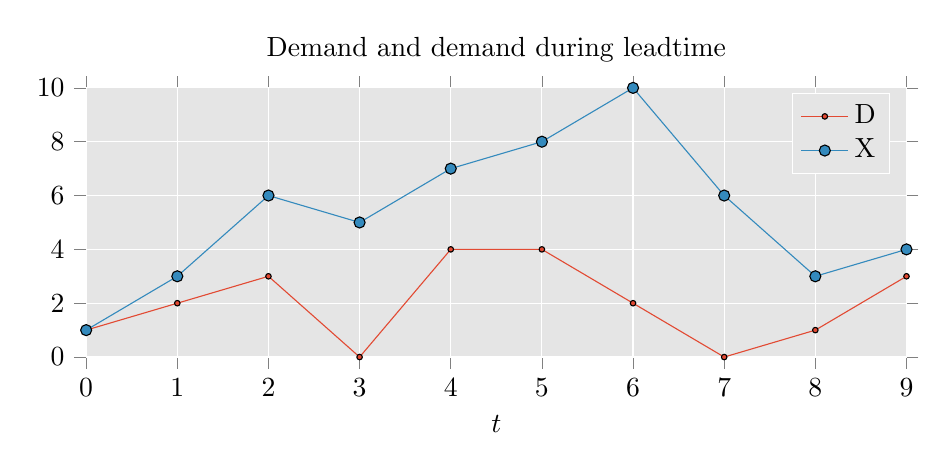
\begin{tikzpicture}

\definecolor{color0}{rgb}{0.886274509803922,0.290196078431373,0.2}
\definecolor{color1}{rgb}{0.203921568627451,0.541176470588235,0.741176470588235}

\begin{axis}[
title={Demand and demand during leadtime},
xlabel={$t$},
xmin=0, xmax=9,
ymin=0, ymax=10,
width=12cm,
height=5cm,
tick align=outside,
xmajorgrids,
x grid style={white},
ymajorgrids,
y grid style={white},
axis line style={white},
axis background/.style={fill=white!89.803921568627459!black},
legend style={draw=white, fill=white!89.803921568627459!black},
legend entries={{D},{X}},
legend cell align={left}
]
\addplot [color0, mark=*, mark size=1, mark options={solid,draw=black}]
table {%
0 1
1 2
2 3
3 0
4 4
5 4
6 2
7 0
8 1
9 3
};
\addplot [color1, mark=*, mark size=2, mark options={solid,draw=black}]
table {%
0 1
1 3
2 6
3 5
4 7
5 8
6 10
7 6
8 3
9 4
};
\end{axis}

\end{tikzpicture}\\
% This file was created by matplotlib2tikz v0.6.0.
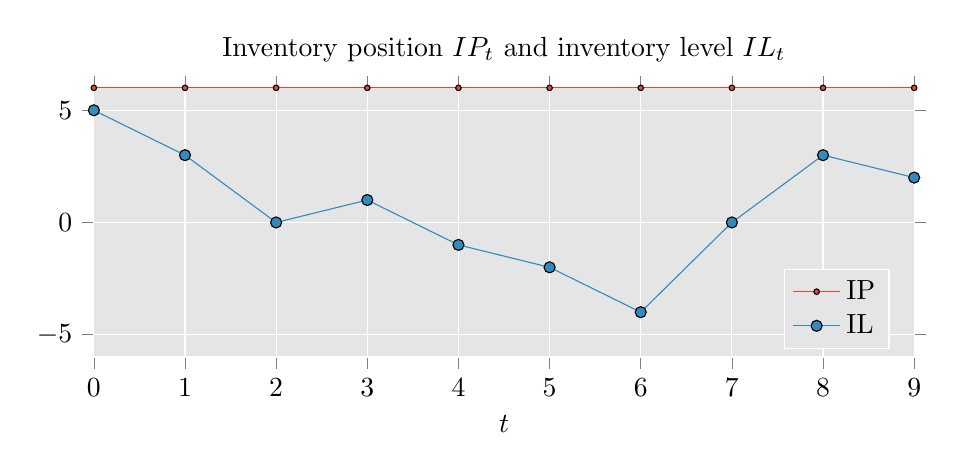
\begin{tikzpicture}

\definecolor{color0}{rgb}{0.886274509803922,0.290196078431373,0.2}
\definecolor{color1}{rgb}{0.203921568627451,0.541176470588235,0.741176470588235}

\begin{axis}[
title={Inventory position $IP_t$ and inventory level $IL_t$},
xlabel={$t$},
xmin=0, xmax=9,
ymin=-6, ymax=6,
width=12cm,
height=5cm,
tick align=outside,
xmajorgrids,
x grid style={white},
ymajorgrids,
y grid style={white},
axis line style={white},
axis background/.style={fill=white!89.803921568627459!black},
legend entries={{IP},{IL}},
legend cell align={left},
legend style={at={(0.97,0.03)}, anchor=south east, draw=white, fill=white!89.803921568627459!black}
]
\addplot [color0, mark=*, mark size=1, mark options={solid,draw=black}]
table {%
0 6
1 6
2 6
3 6
4 6
5 6
6 6
7 6
8 6
9 6
};
\addplot [color1, mark=*, mark size=2, mark options={solid,draw=black}]
table {%
0 5
1 3
2 0
3 1
4 -1
5 -2
6 -4
7 0
8 3
9 2
};
\end{axis}

\end{tikzpicture}
  \end{tabular}
  \caption{Upper panel: demand $D_t$ and demand $X_t$ during the leadtime $L$. Lower panel: inventory position $\IP_t$ and inventory level $IL_t$ as functions of time $t$. Observe that $IL_t = IP_t - X_t.$}
\label{fig:basestock_demand}
\end{figure}

Once we carry out a simulation for $n$ periods, we can estimate the
performance measure. The average  inventory on-hand is
\begin{equation}
  \label{eq:22}
  I = \frac 1n \sum_{t=1}^n \IL_t\1{\IL_t \geq 0} = \frac1n\sum_{t=1}^n \max\{\IL_t, 0\}
\end{equation}
the average backlog  is
\begin{equation}
  B = - \frac 1n \sum_{t=1}^n \IL_t\1{\IL_t < 0} = \frac1n\sum_{t=1}^n \max\{-\IL_t, 0\}
\end{equation}
because $\IL_t<0$ if there are backorders, recall~\eqref{eq:23}. 
The service level is 
\begin{equation}
  \label{eq:22}
  S = \frac 1n \sum_{i=t}^n \1{\IL_t \geq 0},
\end{equation}

For the demand of~\eqref{eq:demand_base}, we define 
\begin{align*}
  I_t &= \max\{\IL_t, 0\}, \\
  B_t &= 0 \min\{\IL_t, 0\}.
\end{align*}
In Figure~\ref{fig:basestock_on_hand} we provide graphs of $I_t$ and $B_t$.

\begin{figure}[tb]
  \centering
  \begin{tabular}[h]{cc}
% This file was created by matplotlib2tikz v0.6.0.
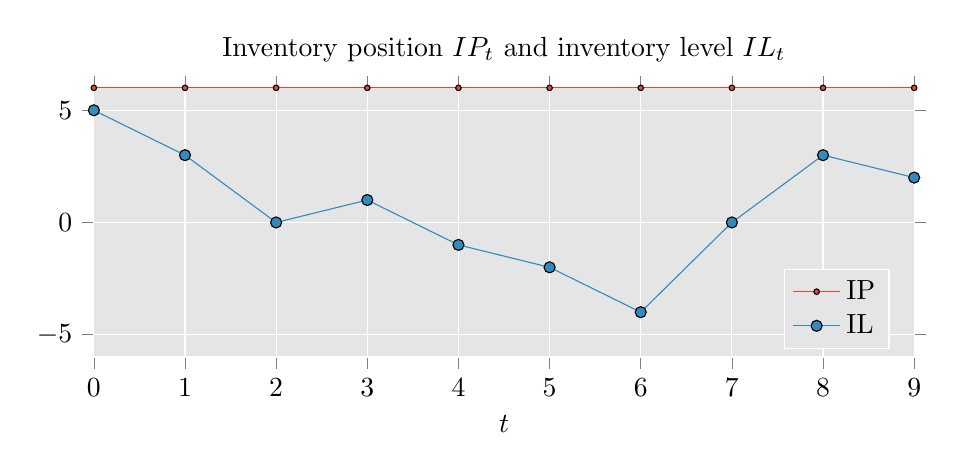
\begin{tikzpicture}

\definecolor{color0}{rgb}{0.886274509803922,0.290196078431373,0.2}
\definecolor{color1}{rgb}{0.203921568627451,0.541176470588235,0.741176470588235}

\begin{axis}[
title={Inventory position $IP_t$ and inventory level $IL_t$},
xlabel={$t$},
xmin=0, xmax=9,
ymin=-6, ymax=6,
width=12cm,
height=5cm,
tick align=outside,
xmajorgrids,
x grid style={white},
ymajorgrids,
y grid style={white},
axis line style={white},
axis background/.style={fill=white!89.803921568627459!black},
legend entries={{IP},{IL}},
legend cell align={left},
legend style={at={(0.97,0.03)}, anchor=south east, draw=white, fill=white!89.803921568627459!black}
]
\addplot [color0, mark=*, mark size=1, mark options={solid,draw=black}]
table {%
0 6
1 6
2 6
3 6
4 6
5 6
6 6
7 6
8 6
9 6
};
\addplot [color1, mark=*, mark size=2, mark options={solid,draw=black}]
table {%
0 5
1 3
2 0
3 1
4 -1
5 -2
6 -4
7 0
8 3
9 2
};
\end{axis}

\end{tikzpicture}\\
% This file was created by matplotlib2tikz v0.6.0.
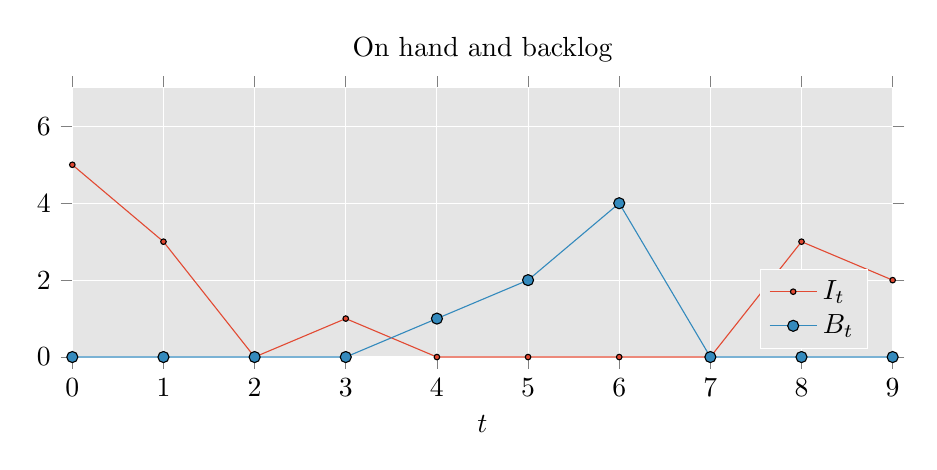
\begin{tikzpicture}

\definecolor{color0}{rgb}{0.886274509803922,0.290196078431373,0.2}
\definecolor{color1}{rgb}{0.203921568627451,0.541176470588235,0.741176470588235}

\begin{axis}[
title={On hand and backlog},
xlabel={$t$},
xmin=0, xmax=9,
ymin=0, ymax=7,
width=12cm,
height=5cm,
tick align=outside,
xmajorgrids,
x grid style={white},
ymajorgrids,
y grid style={white},
axis line style={white},
axis background/.style={fill=white!89.803921568627459!black},
legend entries={{$I_t$},{$B_t$}},
legend cell align={left},
legend style={at={(0.97,0.03)}, anchor=south east, draw=white, fill=white!89.803921568627459!black}
]
\addplot [color0, mark=*, mark size=1, mark options={solid,draw=black}]
table {%
0 5
1 3
2 0
3 1
4 0
5 0
6 0
7 0
8 3
9 2
};
\addplot [color1, mark=*, mark size=2, mark options={solid,draw=black}]
table {%
0 0
1 0
2 0
3 0
4 1
5 2
6 4
7 0
8 0
9 0
};
\end{axis}

\end{tikzpicture}
  \end{tabular}
  \caption{On-hand inventory and backlog as functions of $t$. Clearly, when $B_t=0$ when $I_t>0$, and the other way around. We include a graph of $\IL_t$ for reference.}
\label{fig:basestock_on_hand}
\end{figure}



%%% Local Variables:
%%% mode: latex
%%% TeX-master: "notes_all"
%%% End:
